% A schematic breadth-first exploration tree, not sampled graph data.
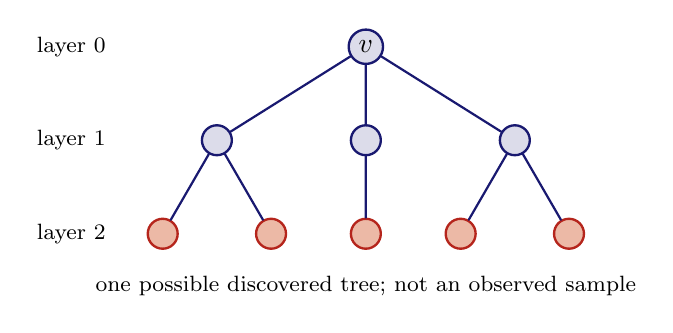
\begin{tikzpicture}[x=0.86cm,y=0.95cm,line cap=round]
  \tikzset{seen/.style={circle,draw=MidnightBlue,fill=MidnightBlue!15,
      inner sep=2pt,minimum size=0.38cm,line width=0.85pt},
    frontier/.style={circle,draw=BrickRed,fill=BrickRed!25,
      inner sep=2pt,minimum size=0.38cm,line width=0.85pt}}
  \node[seen] (root) at (0,2.15) {$v$};
  \node[seen] (a) at (-2.2,0.9) {};
  \node[seen] (b) at (0,0.9) {};
  \node[seen] (c) at (2.2,0.9) {};
  \node[frontier] (d) at (-3.0,-0.35) {};
  \node[frontier] (e) at (-1.4,-0.35) {};
  \node[frontier] (f) at (0,-0.35) {};
  \node[frontier] (g) at (1.4,-0.35) {};
  \node[frontier] (h) at (3,-0.35) {};
  \draw[MidnightBlue,thick] (root)--(a) (root)--(b) (root)--(c)
    (a)--(d) (a)--(e) (b)--(f) (c)--(g) (c)--(h);
  \node[font=\footnotesize,anchor=east] at (-3.7,2.15) {layer $0$};
  \node[font=\footnotesize,anchor=east] at (-3.7,0.9) {layer $1$};
  \node[font=\footnotesize,anchor=east] at (-3.7,-0.35) {layer $2$};
  \node[font=\footnotesize,anchor=north] at (0,-0.78)
    {one possible discovered tree; not an observed sample};
\end{tikzpicture}
